\documentclass[conference,letterpaper]{IEEEtran}
\usepackage[T1]{fontenc}
\usepackage{graphicx}
\usepackage{booktabs}
\usepackage{xcolor}
\usepackage{url}
\usepackage[hidelinks]{hyperref}


\begin{document}

\title{When Agents Wait: Memory Bottlenecks of\\Agent Serving on an Edge LLM Server}

\author{\IEEEauthorblockN{Kai-Cheng Liu}
\IEEEauthorblockA{University of California San Diego\\
CSE 291A, Fall 2026 --- Phase 1 report}}

\maketitle

\begin{abstract}
LLM agents call the model repeatedly, pause for tool calls, and return with a longer conversation each time. We study how a single edge LLM server should admit such agents under a fixed memory budget. On llama.cpp with a 3B model, we build a seeded multi-step agent workload and measure a FIFO scheduler with a fixed concurrency limit $K$ on an Apple M2 Mac and replicate it on an AWS L4 GPU slice. The best fixed $K$ equals the server's slot count on both machines. Admitting more agents than slots evicts their cached context between steps: prompt-cache reuse falls from 65\% to 17--19\% and p95 latency rises 2.0--2.4$\times$ on the Mac but only 1.4$\times$ on the GPU, whose prompt processing is about 4$\times$ faster. Retaining evicted context in host memory or halving KV precision recovers most of the loss. Phase~2 will target memory-bounded retention of agent context across tool calls.
\end{abstract}

\section{Introduction}
LLM agents do not issue one request; they run a loop~\cite{yao2023react}. The agent calls the model, the model asks for a tool such as a search or a code run, the agent waits for the result, and then it calls the model again with the whole conversation so far. Each step's prompt is therefore longer than the last, and between steps the agent leaves the model idle.

A serving system keeps each active conversation in the model's key--value (KV) cache so that it need not reprocess the history at every step, and the size of that cache is fixed by memory. This creates a dilemma. Admitting few agents leaves the hardware idle while they wait on tools; admitting many overflows the memory that holds their conversations, so returning agents find their context evicted and must recompute it. The tension is sharpest on edge servers, where one machine with a few gigabytes serves several agents and memory cannot be added.

Phase~1 asks: \emph{under a fixed memory budget, how do concurrency, context growth and tool waits affect completed agent work, and what is the dominant bottleneck of a simple FIFO baseline?} We answer it on llama.cpp with a 3B model, on an Apple M2 Mac and on an AWS GPU slice.

This report contributes: (1) a seeded multi-step agent workload and an instrumented harness that records every request, task and memory sample; (2) a tuned FIFO baseline with fixed concurrency $K$ on two hardware platforms; (3) evidence that the bottleneck is context eviction once $K$ exceeds the server's slots, shown both by its mechanism and by a causal test that removes it; and (4) a Phase~2 plan for memory-bounded context retention.

\section{Background and Related Work}
\textbf{KV cache and slots.} A transformer server stores the keys and values of every processed token so later tokens need not recompute them. For Llama-3.2-3B this costs 112\,KiB per token in f16. llama.cpp~\cite{llamacpp} divides a fixed KV allocation (\texttt{-c} tokens) evenly among \texttt{-np} \emph{slots}, each serving one request at a time. A slot keeps its last prompt, so a returning conversation whose prefix is still in a slot reuses it (\emph{prompt caching}); otherwise the whole history is processed again. vLLM's PagedAttention~\cite{kwon2023vllm} instead shares one paged pool across requests, and SGLang~\cite{zheng2024sglang} reuses shared prefixes through a radix tree; both target datacenter GPUs.

\textbf{Serving agents.} Agent requests pause for tool calls. InferCept~\cite{abhyankar2024infercept} observes that discarding and recomputing context at each pause wastes 37--40\% of model forwarding time and chooses per request whether to preserve, discard or swap it. Continuum~\cite{li2025continuum} pins an agent's KV cache for a time-to-live during a tool call, set from the reload cost and queueing delay. Both assume a large GPU server. We ask how the same tension appears on a single edge machine with a hard memory budget, where hardware also changes the price of recomputation.

\section{Experimental Setup}
\textbf{Platforms.} Table~\ref{tab:setup} lists both machines. Both run the same llama.cpp build (b11803), the same Llama-3.2-3B-Instruct Q4\_K\_M file (SHA-256 checked) and the same configurations. Micro-benchmarks show their different balance: prompt processing runs at 365--427 tokens/s on the Mac and 1,463--1,651 tokens/s on AWS (3.4--4.2$\times$), while single-request generation runs at 37.5 vs.\ 23.3 tokens/s.

\begin{table}[t]
\caption{Platforms (same build, model and server settings on both)}
\label{tab:setup}
\centering\footnotesize\setlength{\tabcolsep}{4pt}
\begin{tabular}{@{}lll@{}}
\toprule
 & M2 Mac (primary) & AWS (replication) \\
\midrule
Accelerator & Apple M2, 24\,GB & NVIDIA L4-6Q, 6\,GiB \\
 & & (1/4 L4, g6f.2xlarge) \\
Backend & Metal & CUDA \\
Prompt processing & 365--427 tok/s & 1,463--1,651 tok/s \\
Generation, 1 request & 37.5 tok/s & 23.3 tok/s \\
\midrule
Server & \multicolumn{2}{l}{4 slots of 4,096 tokens (\texttt{-c 16384 -np 4})} \\
Memory & \multicolumn{2}{l}{4.1\,GB: weights 2.2, KV 1.8, compute 0.2} \\
\bottomrule
\end{tabular}
\end{table}

\textbf{Workload.} A seeded generator produces four task classes sharing a 200-token system prefix: \emph{chat} (30\%, 1 step, 150--400-token context), \emph{RAG} (20\%, 1 step, 2,000--3,000 tokens), \emph{short agents} (30\%, 3 steps, 0.5--2\,s tool calls returning 100--300 tokens) and \emph{long agents} (20\%, 6 steps, 1--4\,s tool calls returning 200--400 tokens). Each agent step resends the full history, so contexts grow by 200--600 tokens per step. Tasks arrive as a Poisson process at 0.05, 0.1 or 0.2 tasks/s (light load to about 3$\times$ the single-task service rate); each run has 30 tasks and each configuration three seeds.

\textbf{Baseline and controls.} The scheduler admits tasks first-come-first-served up to a concurrency limit $K$; an admitted task keeps its admission through tool calls. Every step generates exactly its fixed output length, so no policy can win by shortening answers. Each run starts a fresh server after two warm-up requests, and llama.cpp's host-RAM prompt cache is disabled so memory equals the allocation above. We report p95 task latency (arrival to completion), throughput, prompt-cache reuse (prompt tokens served from cache), failures by cause, and memory. Failed tasks are kept; runs disturbed by a leftover server process were detected, excluded and rerun.

\section{Baseline: FIFO with Fixed \texorpdfstring{$K$}{K}}
\begin{figure}[t]
\centering
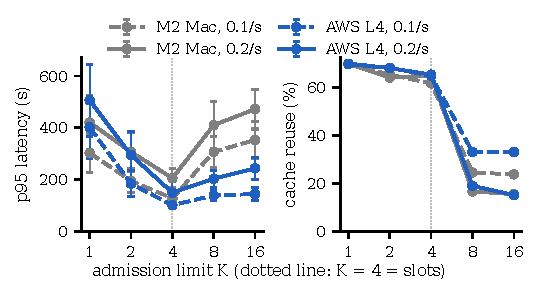
\includegraphics[width=\columnwidth]{fig_ksweep.pdf}
\caption{FIFO baseline over $K$ on both machines (mean of 3 seeds; bars: $\pm$1 std). Latency is lowest at $K=4$, the slot count; above it, cached context is evicted and reuse collapses on both machines.}
\label{fig:ksweep}
\end{figure}

Fig.~\ref{fig:ksweep} shows the result of 90 runs. On both machines latency is lowest when $K$ equals the slot count. Under overload (0.1 and 0.2 tasks/s), $K=4$ cuts p95 latency 2.0--2.4$\times$ relative to $K=1$ on the Mac and 3.4--4.0$\times$ on AWS, where a single request generates slowly; at $K=1$ and 0.2 tasks/s, 6 of 90 AWS tasks exceeded the 600\,s task limit. Raising $K$ beyond the slots makes every metric worse: from $K=4$ to $K=8$ at 0.2 tasks/s, p95 rises from 205 to 410\,s on the Mac and from 149 to 203\,s on AWS. Throughput falls 30\% on the Mac (0.075 to 0.053 tasks/s) and 6\% on AWS (0.090 to 0.084). In almost every configuration 1.7 of 30 tasks fail because a long agent outgrows its 4,096-token slot.

\section{The Bottleneck: Context Eviction}
\textbf{Mechanism.} With $K>4$, more conversations are active than slots exist. A task returning from a tool call usually finds its slot reassigned and its context overwritten, so it reprocesses its whole history. Table~\ref{tab:mech} traces this on both machines: reuse collapses equally, but the cost of rebuilding differs. Each request spends 2.4\,s more on prompt processing on the Mac but 0.6\,s more on AWS, and the long recomputations also slow the generation of requests batched with them (28\% vs.\ 12\%). The cost of exceeding the slot count is roughly the reuse lost, set by the scheduler, times the recomputation cost, set by the hardware.

\begin{table}[t]
\caption{Going from $K=4$ to $K=8$ at 0.2 tasks/s (mean of 3 seeds)}
\label{tab:mech}
\centering\footnotesize
\begin{tabular}{@{}lll@{}}
\toprule
 & M2 Mac & AWS L4-6Q \\
\midrule
Prompt-cache reuse & 65\% $\rightarrow$ 17\% & 65\% $\rightarrow$ 19\% \\
Median prompt time / request & 1.17 $\rightarrow$ 3.55\,s & 0.37 $\rightarrow$ 0.96\,s \\
Generation / request & 12.3 $\rightarrow$ 8.9 tok/s & 12.4 $\rightarrow$ 10.8 tok/s \\
p95 time to first token & 9 $\rightarrow$ 39\,s & 2 $\rightarrow$ 19\,s \\
p95 task latency & 205 $\rightarrow$ 410\,s & 149 $\rightarrow$ 203\,s \\
\bottomrule
\end{tabular}
\end{table}

\textbf{Causal test.} If eviction is the cause, keeping evicted context should remove the penalty. llama.cpp can park evicted prompts in host RAM (\texttt{--cache-ram}). Fig.~\ref{fig:retention} shows $K=8$ on the Mac: a 1\,GB host cache raises reuse from 24\% to 53\% and cuts p95 from 314 to 199\,s within a 6\,GB budget; an 8\,GB cache restores 70\% reuse and matches the best fixed $K$ (128 vs.\ 127\,s) but needs 11.8\,GB. Disabling prompt caching entirely is worse still (375\,s), confirming that reuse is what $K=8$ loses.

\begin{figure}[t]
\centering
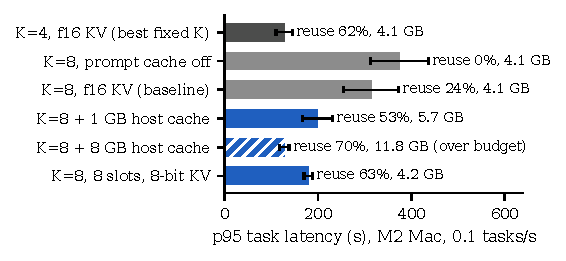
\includegraphics[width=\columnwidth]{fig_retention.pdf}
\caption{$K=8$ on the M2 Mac at 0.1 tasks/s under different memory configurations (mean $\pm$1 std of 3 seeds). Memory is weights plus measured footprint. Retaining context recovers latency; the hatched configuration exceeds the budget.}
\label{fig:retention}
\end{figure}

\textbf{Memory split.} At a fixed KV budget, fewer, larger slots trade concurrency for capacity: 2,048-token slots fail 14 of 30 tasks, 3,072-token slots 9.3, and 4,096-token slots 1.7. An 8-bit KV cache (\texttt{-ctk/-ctv q8\_0}) halves KV memory (952 vs.\ 1,792\,MiB) at unchanged speed, so 8 slots of 4,096 tokens fit in the memory of 4. At $K=8$ this gives every admitted agent its own slot: reuse returns to 63\%, throughput rises 42\% (0.053 to 0.075 tasks/s) and p95 falls from 314 to 179\,s with no extra failures. On 70 quality prompts with greedy decoding, the 8-bit cache gave identical outputs to f16 on all 30 long-context retrieval prompts (0.9k--2.8k tokens) and 20 short-answer prompts; 6 of 20 long free-form answers diverged after a median of 56 tokens into equally fluent text. A repeated f16 run was identical, so these differences come from quantization.

\textbf{Limitations.} The workload is synthetic: filler text, with tool delays and step counts chosen rather than measured. The slot-eviction mechanism is specific to servers with fixed per-request slots such as llama.cpp; a paged pool~\cite{kwon2023vllm} would degrade differently. p95 over 30 tasks is noisy, so we claim only differences larger than one standard deviation, and overload runs end before a steady state. The memory budget on the Mac's unified memory is enforced by configuration, not hardware.

\section{Phase 2 Plan}
Section~V shows that admitting more agents than slots pays off only if their context survives tool calls, and that the right amount of retention depends on memory and on hardware. Phase~2 will therefore build \emph{memory-bounded context retention}: admit more agents than slots, and when an agent enters a tool call, decide whether to keep its context in its slot, park it in a bounded store outside the GPU (llama-server can save a slot's KV state to a file and restore it), or drop it and recompute later. The decision weighs the cost of recomputing the context, measured per platform from its prompt-processing rate, against the cost of holding memory that waiting agents could use, given the agent's expected tool time. Free slots go first to agents whose context is resident. Total memory, including parked context, stays within the 6\,GB budget. Unlike InferCept~\cite{abhyankar2024infercept} and Continuum~\cite{li2025continuum}, which target paged GPU servers, the policy works within fixed slots on one edge machine, enforces a hard total memory budget, and adapts its decisions to a recomputation cost that differs 4$\times$ between our two platforms.

We will compare against three tuned baselines: FIFO at the best fixed $K=4$; $K=8$ with llama.cpp's built-in 1\,GB host cache (LRU, no knowledge of agents); and 8 slots with an 8-bit KV cache. A fixed time-to-live in the style of Continuum serves as an ablation. Evaluation uses held-out workload seeds (1000+), both platforms, the current mix and a variant with longer tool calls (5--30\,s), and reports p95 latency per task class, throughput, failures, peak memory including parked context, and the policy's save/restore overhead. We expect larger gains on the Mac, where recomputation is slower, and smaller but positive gains on AWS.

\bibliographystyle{IEEEtran}
\bibliography{refs}

\end{document}
